%--------------------------------------
% Create title frame
\titleframe

%--------------------------------------
% Table of contents
\begin{frame}{Overview}
  \setbeamertemplate{section in toc}[sections numbered]
  \tableofcontents[hideallsubsections]
\end{frame}

\section{Introduction}

\begin{frame} {Lecture objectives}
    \begin{itemize}
        \item Formulate the real-time optimization problem
        \item Understand it's connection with other control problems
        \item Practice linear programming modeling and gain intuition in the solutions' properties
        \item Understand the benefits of optimization with respect to simple rules
    \end{itemize}
\end{frame}

\begin{frame} {What is real-time optimization}
\begin{itemize}
\item Real-time optimization is a secondary control layer that sends reference power set-points, or targets, to devices to 
\begin{itemize}
    \item minimize the system's operation cost
    \item restore margins for droop controllers (primary control layer). 
\end{itemize}  
\item Power set-points are mainly for active power  
\begin{itemize}
    \item but may also be reactive power set-points in case voltage must be regulated (but this is out of the scope of this lecture).
\end{itemize}
\item Lower-level controllers receive these set points and regulate currents and voltages to satisfy them. They may, however, leave an error because of instantaneous changes in the environment and slow system dynamics that do not allow frequent set point changes.
\end{itemize}
\end{frame}

\begin{frame}{Frequency control in one schematic}
    \begin{center}
        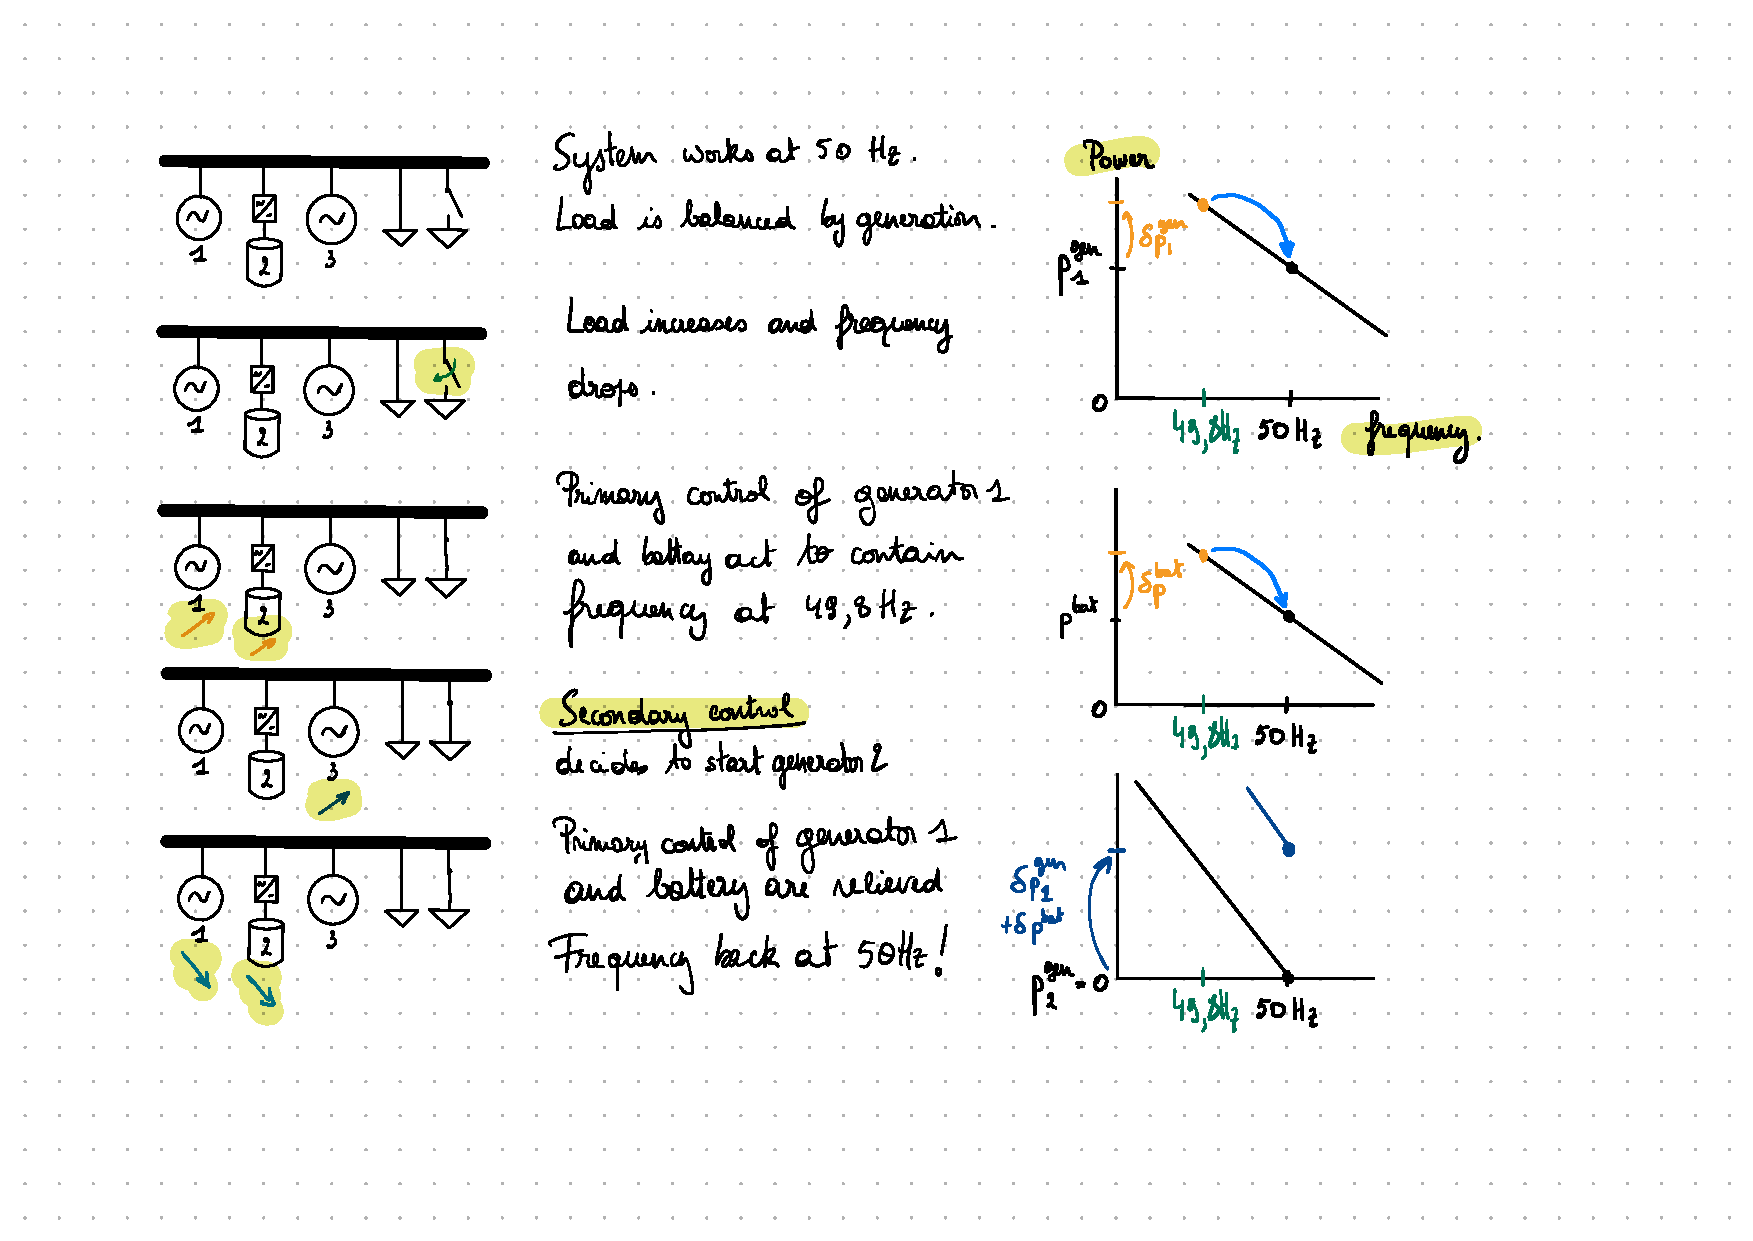
\includegraphics[width=0.75\textwidth, clip, trim=2cm 2cm 2cm 1cm]{images/primary_control.pdf}    
    \end{center}
\end{frame}

\begin{frame} {Methods}
\begin{itemize}
\item  Real-time optimization can be accomplished through different methods. 
\item Many controllers use basic if-then rules, i.e., \textbf{rule-based controllers}. 
\item Although these rules are simple and easy to understand, they are not ideal for microgrids with numerous devices or complex grid interaction mechanisms. 
\item In such cases, \textbf{optimization-based control} is better suited. We will compare the two approaches in a simple example.
\end{itemize}
\end{frame}

\begin{frame}{Control time scale}
    Real-time operation means that decisions are taken frequently, every $\Delta t$ seconds.
    \begin{itemize}
        \item An upper bound on $\Delta t$: renewable generation that can vary significantly within a few seconds, or abrupt load changes
        \item A lower bound on $\Delta t$: lower-level control loops (e.g., power point tracking) must have the time to converge to avoid interference between control levels
    \end{itemize}

    We will assume that $\Delta t \approx 1 s$.
\end{frame}

\begin{frame}{Notation}
\begin{itemize}
    \item Lowercase symbols are control variables
    \item Uppercase symbols and Greek letters are fixed values (parameters or measurements)
    \item Subscript $t$ is a time index, sometimes omitted to simplify reading
    \item Subscript $d$ is a device index, omitted if there is only one device
    \item Superscript $PV$ refers to a photovoltaic system
    \item Superscript $bat$ refers to a battery storage system
    \item Superscript $load$ refers to a load
    \item Superscript $gen$ refers to a generator
\end{itemize}
    

\end{frame}


\section{Off-grid microgrid use case illustration}
\begin{frame}{Off-grid microgrid}
    \begin{multicols}{2}
        
    
    Let us consider an off-grid microgrid with photovoltaic panels with an installed capacity of $C^{PV}$, a stationary battery, a backup diesel generator, and an uncontrollable load. For now, we are neglecting the electrical grid connecting these devices.

    \begin{center}
    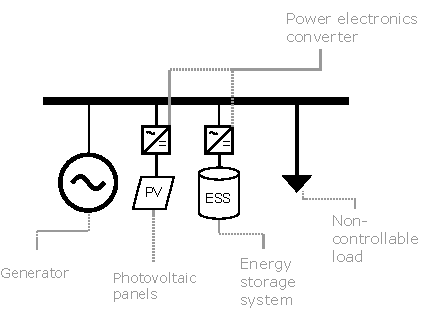
\includegraphics[width=0.5\textwidth]{images/off_grid_1.pdf}        
    \end{center}
\end{multicols}
\end{frame}

\begin{frame}{Microgrid state}
At time $t$, the state of the microgrid can be described by
\begin{enumerate}
 \item the power consumed by the load $P^{load}_t$ % TODO macros
 \item the maximum power that the PV panels can produce $\bar{P}^{PV}_t \leq C^{PV}$. 
 \item the state of charge of the battery, $S_t$
 \item the maximum power the battery can deliver $\bar{P}^{bat}_t$ or consume $\underline{P}^{bat}_t$. 
 \item (the ON/OFF state of the generator and the duration in that state.)
\end{enumerate}
This state must thus be partly measured and partly estimated.
\end{frame}

\begin{frame}{About the Maximum Power Point $\bar{P}^{PV}_t$}

    %\begin{multicols}{2}
    This quantity is usually unknown and is approached when the inverter is working at its maximum power point (MPP). As soon as a curtailment instruction is given, i.e., a set point below the maximum power point, the actual MPP is unknown and must be estimated. 

    \begin{center}    
    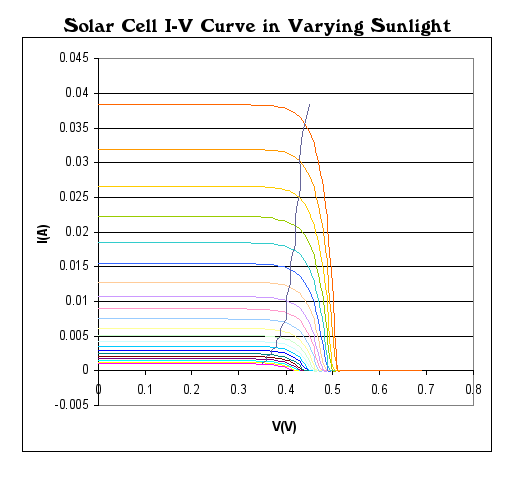
\includegraphics[width=0.35\textwidth]{images/Solar-Cell-IV-curve-with-MPP.png}%\\
    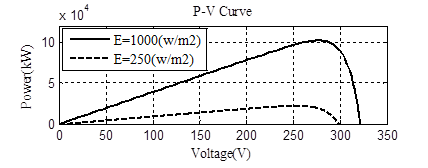
\includegraphics[width=0.55\textwidth]{images/Power-voltage_(P_-V)_curve.png}    
    \end{center}

    %\end{multicols}

%TODO provide references for MPP estimation.
\end{frame}
\begin{frame}{The maximum battery power}

The maximum power the battery can deliver $\bar{P}^{bat}_t$ or consume $\underline{P}^{bat}_t$ varies with time since it is a function of the state of charge (SoC), the temperature, etc. This information comes from the battery management system (BMS).
    
\end{frame}

\begin{frame}{Generator}
 A generator may need a nonnegligible minimum time to start up, and too frequent starts and stops should be avoided to limit wear and tear.
 There is a minimum stable generation level and ramping constraints.

 We will consider a simple model in this lecture.
\end{frame}




\subsection{Rule-based controller}

\begin{frame}{Control decisions and objective}

Since the load is not controllable, the \alert{control decisions} are 
\begin{itemize}
    \item the battery's charging or discharging power $p^{bat}_t$
    \item the generator's power $p^{gen}_t$
    \item if needed, a curtailment instruction for the PV panels $p^{PV}_t$
\end{itemize}
Let $$p_t = (p^{bat}_t, p^{gen}_t, p^{PV}_t).$$


The \alert{objective} is to maximize the energy harvested from the PV panels and use the diesel generator as little as possible. 

\end{frame}

\begin{frame} {Rule-based controller}

\tiny

Input: the microgrid state.
\begin{multicols}{2}
   \begin{algorithmic}
    \State Compute the imbalance between the load and the maximum PV generation $\delta_t = P^{load}_t - \bar{P}^{PV}_t$
    \If{$\delta_t > 0$}
    \LComment{Excess load, discharge first, then use the generator}
        \State $p^{PV}_t \gets \bar{P}^{PV}$ 
        \Comment{Produce the maximum with PV generation}
        \If {$\bar{P}^{bat}_t > \delta_t$}
        \State $p^{bat}_t \gets \delta_t$ %
        \State $p^{gen}_t \gets 0$ % 
        \State $\delta_t \gets 0$
        \Else{}
                \State $p^{bat}_t \gets \bar{P}^{bat}_t$ 
                \Comment{Discharge the battery at full power}
                \State $\delta_t \gets \delta_t - p^{bat}_t$
                \Comment{Use the generator to cover the remaining load}
            \If {$\bar{P}^{gen}_t > \delta_t$}
                \State $p^{gen}_t \gets \delta_t$
            \Else
                \LComment{Run the generator at full power}
                \State $p^{gen}_t \gets \bar{P}^{gen}_t$
                \State $\delta_t \gets \delta_t - p^{gen}_t$
                \Comment{The load exceeds the maximum generation capacity}
            \EndIf
        \EndIf
    \Else {}
        \LComment{Excess PV, charge first then curtail}
        \State $p^{gen}_t \gets 0$ 
        \Comment{Shut down the diesel generator}
        \If {$\underline{P}^{bat}_t > -\delta_t$}
            \State $p^{bat}_t \gets \delta_t$
            \State $p^{PV}_t \gets \bar{P}^{PV}$ 
            \Comment{No need to curtail}
        \Else {}
            \State $p^{bat}_t \gets -\underline{P}^{bat}_t$
            \Comment{Charge the battery at full power}
            \State $\delta_t \leftarrow \delta_t - p^{bat}_t$
            \State $p^{PV}_t \gets \bar{P}^{PV}_t + \delta_t$
            \Comment{Curtail excess PV generation}
        \EndIf {}
        \State $\delta_t \gets 0$
        \EndIf
    \State $p_t \gets (p^{bat}_t, p^{gen}_t, p^{PV}_t)$
    \Return $p_t, \delta_t$
\end{algorithmic}
\end{multicols}
\end{frame}

\begin{frame}{Comments}
    A positive $\delta_t$ returned value indicates an emergency measure should be taken to shed some load. 
    
    This should, however, not happen if the system and the microgrid's electric protections are properly designed. 
\end{frame}

\begin{frame}[label={RBC_example}]{Graphical view}
\begin{multicols}{2}
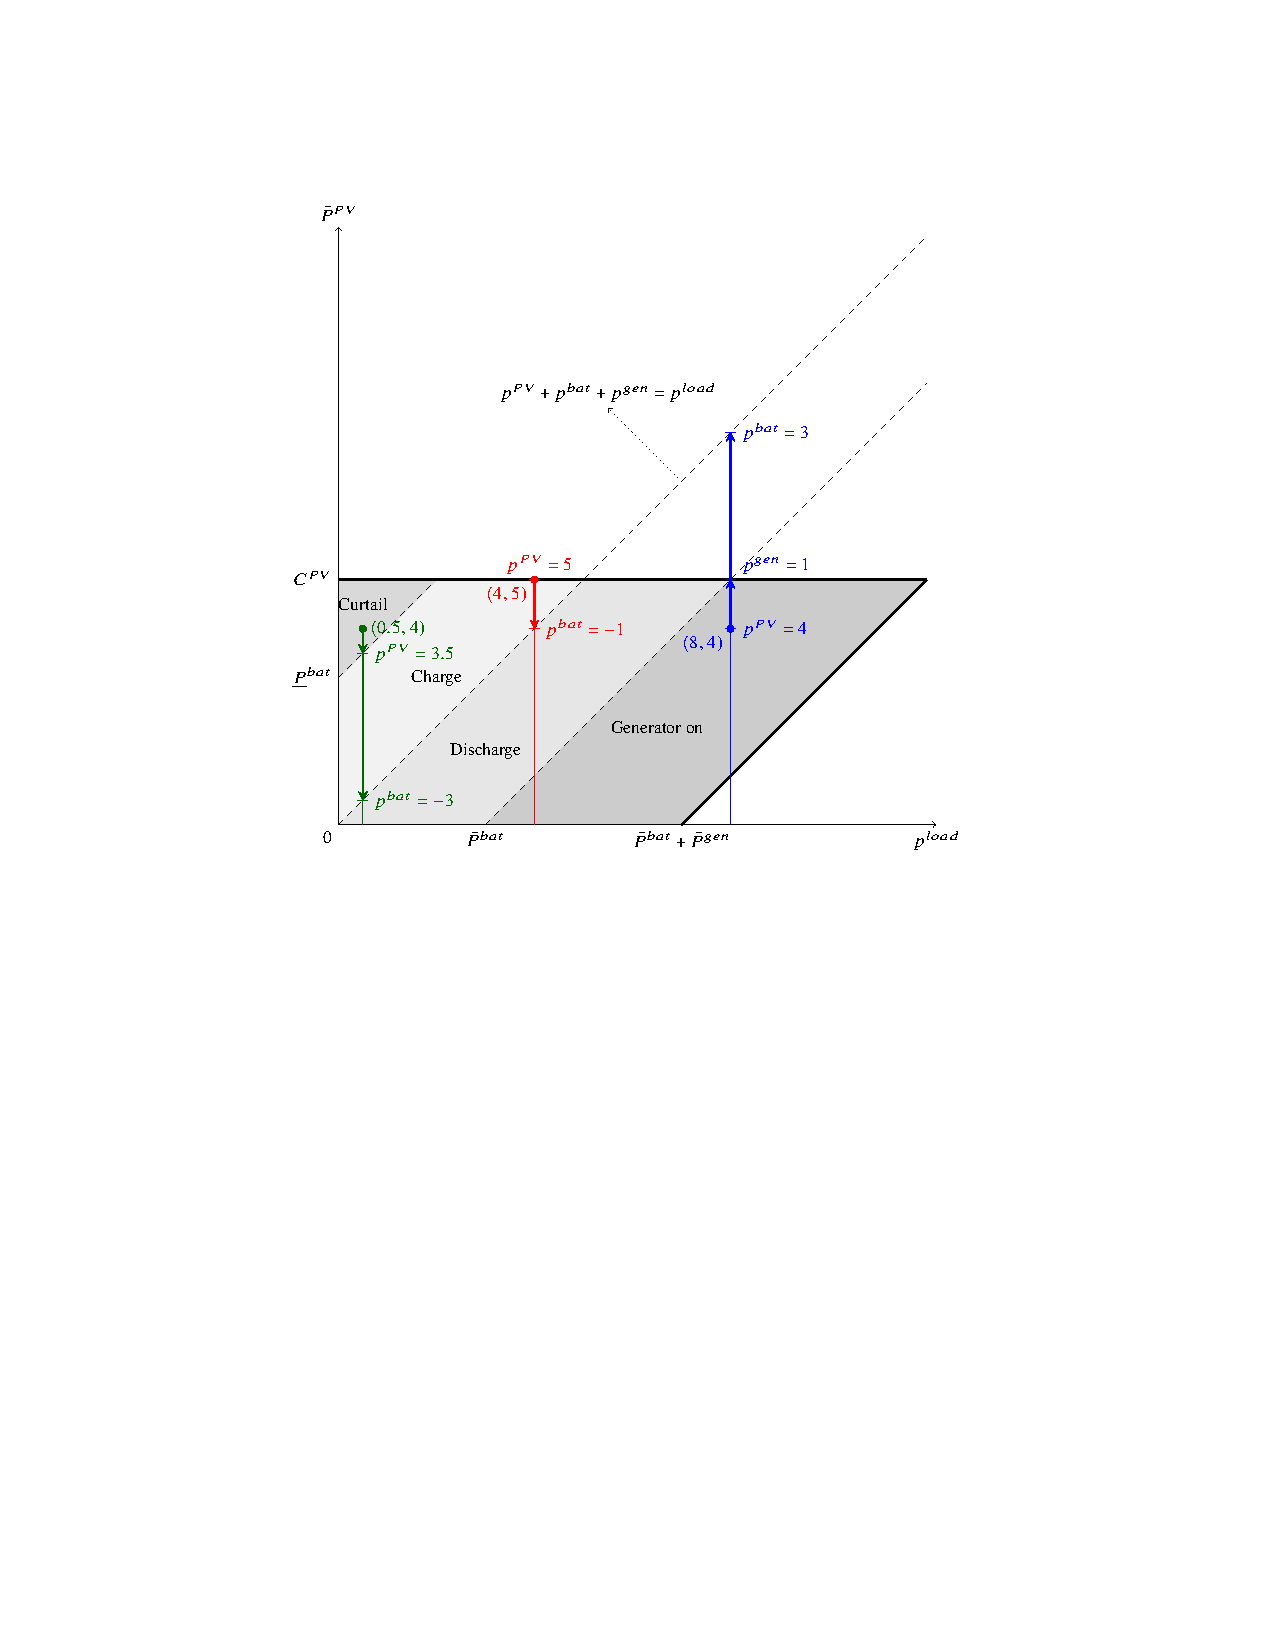
\includegraphics[width=0.5\textwidth]{images/RB_graphical.pdf}
Illustration of the rule-based controller when $C^{PV} > \underline{P}^{bat}_t > 0$ and $\bar{P}^{bat}_t >0$ (index $t$ omitted in the graph).  Three $(p^{load}, \bar{P}^{PV})$ operating points are higlighted in green $(0.5,4)$, red $(4,5)$ and blue $(8,4)$, with the corresponding setpoints for $p^{PV}$, $p^{bat}$, and $p^{gen}$.
\end{multicols}
\end{frame}

\subsection{Optimization-based controller}

\begin{frame}[allowframebreaks]{Optimization-based controller}
An alternative way of solving this problem is to state the problem as a linear program. 
\begin{subequations}
	\label{eq:RT1}
    \begin{align}
    \min        \quad  & \pi^{gen} p^{gen}  + \epsilon p^{bat}\\
    \text{s.t.} \quad  & p^{PV}+p^{bat}+p^{gen} = P^{load} \\
                    & p^{PV} \leq \bar{P}^{PV} \\
                    & -\underline{P}^{bat} \leq p^{bat} \leq \bar{P}^{bat} \\
                    & p^{gen} \leq \bar{P}^{gen}\\
                    & p^{gen}, p^{PV} \geq 0
    \end{align}
\end{subequations}

With $\epsilon < \pi^{gen}$, the objective function favors PV generation (free), then the battery, then the generator. 

\begin{itemize}
    \item The coefficient $\epsilon$ is somewhat virtual but could also model a battery usage cost or a value degradation when $p^{bat} > 0$.
    \item In case of excess PV, charging the battery is preferred over curtailment since having $p^{bat} < 0$ decreases the objective. 
    \item Without this coefficient, the optimization problem would consider charging the battery or curtailing renewable generation as equivalent solutions.
\end{itemize}

While the rule-based controller algorithm is relatively concise, Problem~\eqref{eq:RT1} is even more compact. 
However,
\begin{itemize}
    \item It needs a solver. Nowadays, open-source and commercial solvers are very efficient and easy to interface with mainstream programming languages. 
    \item Such small optimization problems are solved in a few milliseconds. 
    \item wrong parameters may cause infeasibility. 
\end{itemize}
\end{frame}


\begin{frame}{Handling infeasibility}
For instance, if the load exceeds the maximum generation capacity, the rule-based algorithm outputs the best possible solution and a non-zero $\delta_t$. 
In contrast, Problem~\eqref{eq:RT1} returns no solution and an error message. 

It is, however, easy to make the problem more robust: 
\begin{itemize}
    \item add slack variables to the power balance constraint: let $p^+ \geq 0$ and $p^- \geq 0$ represent an excess of generation and a shortage of generation, respectively. 
    \item replace the power balance constraint by $p^{PV}+p^{bat}+p^{gen} + p^-= P^{load} + p^+$
    \item add a term $V (p^+ + p^-)$ to the objective function, with a parameter $V$ large.
\end{itemize} 

This leads to Problem~\eqref{eq:RT2}.
\end{frame}

\begin{frame}{Formulation as a feasibility problem}
\begin{subequations}
	\label{eq:RT2}
\begin{align}
\min        \quad  & \pi^{gen} p^{gen}  + \epsilon p^{bat} \color{red}{+ V (p^+ + p^-)} \label{eq:obj_2}\\
\text{s.t.} \quad  & p^{PV}+p^{bat} +p^{gen} {\color{red}+ p^-}  = P^{load} {\color{red} + p^+}  \label{eq:bal_2} \\
                   & p^{PV} \leq \bar{P}^{PV}  \label{eq:PV_2}\\
                   & -\underline{P}^{bat} \leq p^{bat} \leq \bar{P}^{bat}  \label{eq:bat_2}\\
                   & p^{gen} \leq \bar{P}^{gen}  \label{eq:gen_2}\\
                   & p^{gen}, p^{PV}  \geq 0  \label{eq:nonneg_2}
\end{align}
\end{subequations}


\end{frame}

\section[General formulation of the optimization-based controller]{General formulation of the\\ optimization-based controller}

\begin{frame}[allowframebreaks]{Battery limits and SoC update}

    The battery management system (BMS) usually provides up-to-date limits to the battery power $p^{bat}$ that reflect not only the inverter capability but also the SoC of the battery, the impact of the battery temperature, etc.
    
    As a security, the SoC $s^{bat}$ can be tracked with 
    $$s^{bat}_{t+\Delta t} = S^{bat}_{t} + p^{bat}_t  \Delta t$$
    and bounded by SoC limits
    $$ \underline{S}^{bat} \leq s^{bat}_{t+\Delta t} \leq \bar{S}^{bat}.$$

    Since $\Delta t$ is small, the amount of energy charged or discharged is also small compared to the storage size but may become significant close to the SoC limits.
    This type of constraint is optional here but mandatory in a planning stage where the time step is on the order of a minute.

    However, this state evolution constraint is inaccurate when accounting for charge and discharge efficiencies.
\end{frame}

\begin{frame}[allowframebreaks]{Charge and discharge efficiencies}
    To account for charge and discharge efficiencies, we can subdivide the battery power into charge and discharge powers as 
    $$ p^{bat} = p^{bat, charge} - p^{bat, discharge}$$
    with $p^{bat, charge} \geq 0$ and $p^{bat, discharge} \geq 0$.

    Then, the SoC update can be rewritten as
    $$s^{bat}_{t+\Delta t} = S^{bat}_{t} + p^{bat, charge}_t  \eta^{charge} \Delta t - p^{bat, discharge}_t / \eta^{discharge} \Delta t $$
    with $\eta^{charge} \in [0,1]$ and $\eta^{discharge} \in [0,1]$.

    \begin{itemize}
        \item Multiplying $p^{bat}$ by an average efficiency $\eta \in [0,1]$ would be fine for charging, but discharging the battery would lead to a problem in the energy balance.
        \begin{block}{Example}
            Assume $p^{bat} = -10 kW$, although the battery generates 10 kW over $\Delta t$, it will be discharged by only $10 kW \Delta t \times \eta$.    
        \end{block}
        \item The optimizer may lead to a solution with simultaneous charge and discharge. 
        This can be avoided by adding constraints, such as $p^{bat, charge} \times p^{bat, discharge} = 0$, or introducing binary variables. The problem becomes either a non-linear program (NLP) or a mixed-integer linear program (MILP).
        \item Non-linear efficiencies.
    \end{itemize}
\end{frame}

\begin{frame}[allowframebreaks]{Non-linear efficiency}

    \begin{center}
        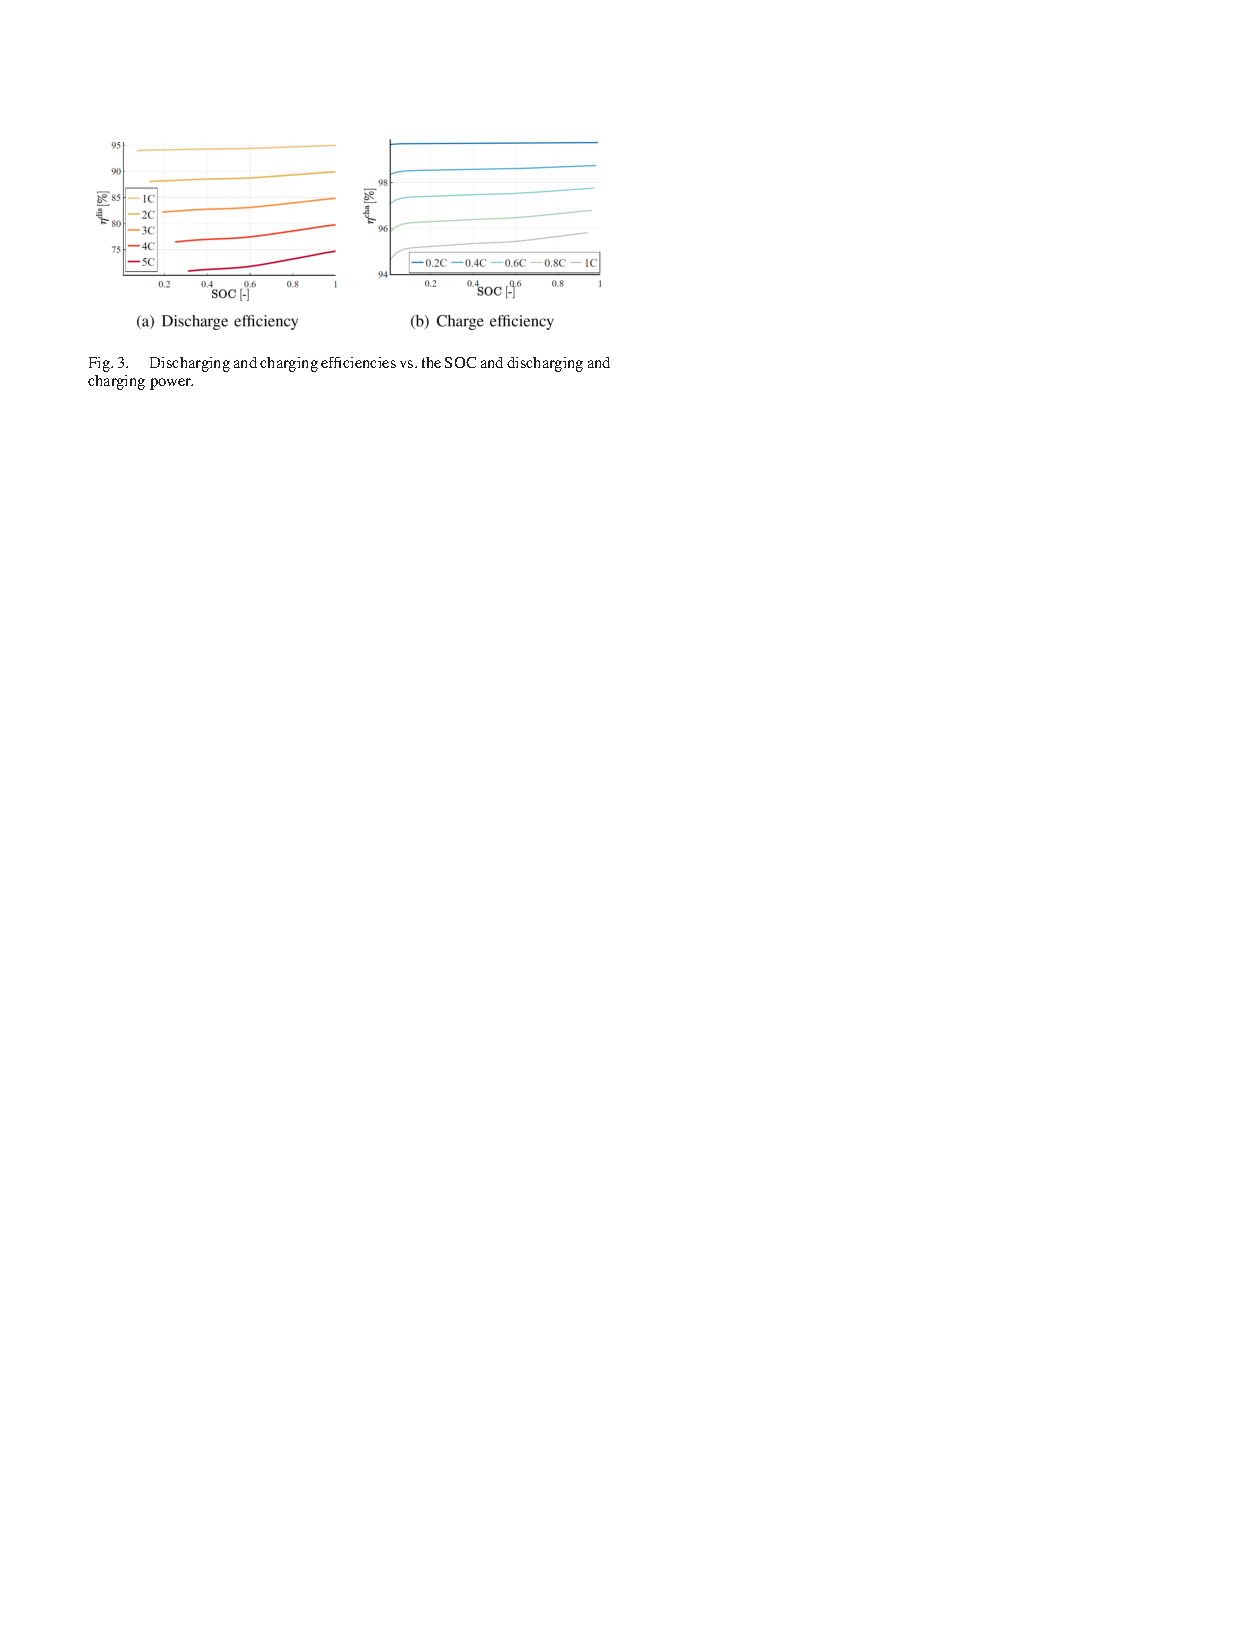
\includegraphics[width=0.6\textwidth]{images/Non-Ideal_Linear_Operation_Model_for_Li-Ion_Batteries.pdf} \\
        From the reference cited on the next slide.
    \end{center}
    
    It is possible to approximate non-linear efficiency and also maximal charge and discharge power using linear models.
    They depend on the SoC and the power. 
    
    In the article below, a convex envelope of the operating region is employed to obtain a linear model with a moderate increase in the number of variables and solution time.

    \textit{Gonzalez-Castellanos, A. J., Pozo, D., \& Bischi, A. (2019). Non-ideal linear operation model for li-ion batteries. IEEE Transactions on Power Systems, 35(1), 672-682.}

    Remark: converter inefficiency may also lead to a low charge or discharge efficiency at very low power.
\end{frame}


\begin{frame}[allowframebreaks]{Grid connection}
    A grid connection allows importing $p^{imp}_t$ or exporting $p^{exp}_t$ power to the grid but also increases the system's inertia, offers the possibility to provide ancillary services, etc.
    \begin{center}
    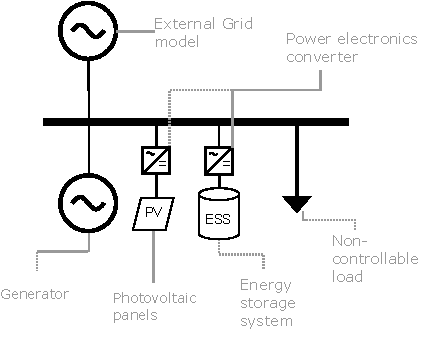
\includegraphics[width=0.6\textwidth]{images/grid_tied_1.pdf}
    \end{center}
    
    The power balance must be updated to 
    $$p^{PV}+p^{bat} +p^{gen} + p^- {\color{red} + p^{imp}}  = p^{load} + p^+ {\color{red} + p^{exp}} $$
    but import $0 \leq p^{imp} \leq \bar{P^{imp}}$ and export limits $0 \leq p^{exp} \leq \bar{P^{exp}}$ must be considered. 
    They model either a physical or a contractual limit.

    The objective function must also be updated to consider the import $\pi^{imp}_t$ and export $\pi^{exp}_t$ prices : 
    $$\pi^{gen} p^{gen}  + \epsilon p^{bat} {\color{red}{+ \pi^{imp}_t p^{imp}_t - \pi^{exp}_t p^{exp}_t}} + V (p^+ + p^-)$$

    Other aspects may also be invoiced, such as the peak power or the power factor. However, they are usually estimated over a period of several weeks.
\end{frame}


\begin{frame}[allowframebreaks]{Sets of devices}
In the general case, we can have an arbitrary number of devices of each type.
\begin{block}{Example}
Instead of one PV inverter, we now have a set $\mathcal{D}^{PV}$ of PV inverters.
\end{block}

Straightforward adaptations: 
\begin{itemize}
    \item Sum over all these devices in the constraints and objective
    \item Express device-level constraints for all devices
\end{itemize}

\begin{block}{Example}
\begin{itemize}
    \item Replace $p^{PV}$ by $\sum_{d \in \mathcal{D}^{PV}} p^{PV}_d$ in the balance equation.
    \item $p^{PV}_d \leq \bar{P}^{PV}_d \quad \forall d \in \mathcal{D}^{PV}$.
\end{itemize}
    
\end{block}

A less obvious adaptation is related to the power-sharing among devices of the same type.

Open question: do you see other adaptations? 
\end{frame}

\begin{frame}[allowframebreaks]{Power sharing between devices of the same type}
    Devices of the same type may \textit{differ} by some parameters such as efficiencies and costs. 
    In that case, the optimizer will decide to use the devices by \alert{merit order} (lowest cost first) unless some technical constraints lead to other solutions.

    If devices are \textit{perfectly equivalent}, then \alert{multiple solutions} may be optimal.
    It is then up to the user to decide whether he wants to share the power equally or rather shut down a maximum of devices, or ...
    
    \begin{block}{Example}
        Share the curtailment between two equivalent PV installations (same peak power, orientation, and inverter).    
    \end{block}
    A possibility is to solve the optimization problem first and then to fix all decisions except those under consideration.
    Then rerun a second problem by forcing the original objective to take the optimal value and changing the objective to reflect the sharing goal.
    For our example a new objective could be $\sum_{d \in\mathcal{D}^{PV}} {p^{PV}_d}^2$.

    Let $$z^{(2), \star} = \min \eqref{eq:obj_2} \quad \text{s.t.} \eqref{eq:bal_2} - \eqref{eq:nonneg_2}$$
    and $$p^{(2), \star} = \arg \min \eqref{eq:obj_2} \quad \text{s.t.} \eqref{eq:bal_2} - \eqref{eq:nonneg_2}.$$
    \begin{subequations}
        \label{eq:RT3}
    \begin{align}
    \min        \quad  & \sum_{d \in\mathcal{D}^{PV}} {p^{PV}_d}^2 \label{eq:obj_3}\\
    \text{s.t.} \quad  & \eqref{eq:bal_2} - \eqref{eq:nonneg_2}  \label{eq:const_3} \\
                       & \pi^{gen} p^{gen}  + \epsilon p^{bat} + V (p^+ + p^-) = z_2^\star \label{eq:eq_obj_3}\\
                       & (p^{gen} = p^{gen, (2), \star})\\
                       & (p^{bat} = p^{bat, (2), \star})
    \end{align}
    \end{subequations}

\end{frame}


\begin{frame}{Device availability}
    A device may be temporarily under maintenance, or, for an electric car, it may not be connected or not be available for recharging.
    This can be handled either:
    \begin{itemize}
        \item by removing explicitly the related variables from the problem formulation
        \item by forcing them to an adequate value (e.g. $\bar{P}^{charge}_t = 0$)        
    \end{itemize}
\end{frame}

\begin{frame}[allowframebreaks]{Long-term targets}
    Let's assume we have a storage device, and for some reason, we want to have it charged in a given amount of time.
    \begin{block}{Example}
        It is 9 AM, a car is charged at $50\%$, and we want it to be charged at $80\%$ at 5 PM.
    \end{block}

    Include a penalty in the objective function on the difference between the SoC $s^{bat}_{t+\Delta t}$ and the target SoC $S^{bat, \dagger}$:
    $$W (s^{bat}_{t+\Delta t} - s^{bat, \dagger})$$
    with $W$ a coefficient wisely chosen.

    Question: what will be the effect of this term?

    A more involved method is proposed in \\
    \textit{Dumas, J., Dakir, S., Liu, C., \& Cornélusse, B. (2021). Coordination of operational planning and real-time optimization in microgrids. Electric Power Systems Research, 190, 106634.}
    where a value function is extracted from a planning problem (optimization over several hours) and integrated into the objective function to reach a trade-off between instantaneous revenues and long-term rewards.
\end{frame}




\begin{frame}{Avoiding multiple solutions}
    Besides having sets of similar devices that may lead to several equivalent solutions, other less intuitive reasons may also lead to multiple solutions.

    We thus need rules for lifting indeterminacies, and we can follow a similar approach to the one of presented for handling several equivalent devices.
\end{frame}

\begin{frame} {Avoid oscillations and large set point changes} 

    Let $P \leftarrow p_{t-\Delta t}$.
    
    To avoid large variations of the control actions, we can for instance impose new constraints 
    $$| p_t - P| \leq \Delta P \Delta t$$
    with $\Delta P$, a parameter to limit variations expressed in power units per second.

    Question: How do we model the absolute value in a linear program?
\end{frame}


%\begin{frame}[allowframebreaks]{Hands on}
%    In the Google Colab template provided, 
%    \begin{enumerate}
%        \item (implement the rule-based controller (RBC), test the values of the example of slide \ref{RBC_example})
%        \item implement the optimization-based controller of Problem~\eqref{eq:RT1}
%        \item implement the SoC update constraint with perfect efficiency
%        \item implement the imperfect charge and discharge efficiencies
%        \item add a grid connection with import and export prices and import/export limits
%        \item add an electric vehicle to your problem with a long-term charge target.
%    \end{enumerate}
%    \begin{itemize}
%        \item Test each of the controllers above using the time series of PV generation and load provided.
%        \item Report the total cost, the PV energy curtailed, and the usage of the battery.
%        \item Bonus: find an input state that makes Problem~\eqref{eq:RT1} infeasible, implement Problem~\eqref{eq:RT2}, and compare.
%    \end{itemize}
%    
%\end{frame}
